\section{Experiments results}\label{sec:expr}

Our tool MEB (Multi Estimation Based Backbones Extraction) was built with C++ using minisat\cite{MINISAT} as the underlying SAT solver. It contains the $\NBL_u$ computing and $\HDBS$ computing proposed in Section 3. The experiments were conducted on a cluster of IBM iDataPlex 2.83 GHz, each instance was running with a timeout of 1 hour and memory limit of 8 GB.

Since SAT solver is an oracle in the extraction of backbones, calling a SAT solver and waiting for results takes the majority of CPU time. We set up two metrics for comparisons, total SAT solvers CPU time(st) and SAT solver calls number(sc).

\subsection{Experimental Strategies}

Earlier work\cite{JLM15} carried out numerous evaluations of different backbones extraction Algorithms. It shows that Core Based algorithms is more consistent and efficiency for large scale instances. Hence, we compared MEB against CB from the st and sc aspects.
In order to present an overall evaluations, we focus on the following cluster of benchmarks: (1) Maximal Satisfiable Subset(MSS) from unsatisfiable instances. (2) Satisfiable instances from SAT competition\footnote{http://www.satcompetition.org/}. (3) Easy satisfiable instances from SATLIB\footnote{http://www.cs.ubc.ca/~hoos/SATLIB/benchm.html}.

The reason we choose MSS instances is that due to the theory of satisfiability, the density of backbones in MSS instances will be higher on average. It helps reveal how MEB and CB performances with a higher density backbones.
Easy satisfiable instances are chosen to apprise the total SAT calls number without a possibility of timeout or memory leak. In other words, we want to make sure that each instances in this cluster is easy enough for MEB and CB to get results in blink.
The selected satisfiable instances are all from industrial and is guarantied that both MEB and CB is able to finish computing under the resource limits.

\subsection{MSS Extraction Experimental Results}
In this section, the effectiveness of MEB and CB for MSS instances are presented.
\begin{definition}[Maximal Satisfiability Sub-formulae(MSS)]
Given an unsatisfied propositional formula $\Phi$, a sub-formula $\Phi'\subseteq\Phi$ is called a Maximal Satisfiability sub-formula (MSS) of $\Phi$ iff $\Phi'$ is satisfiable and $\Phi'\wedge(\phi\in(\Phi\setminus\Phi'))$ is unsatisfiable.
\end{definition}

MSS instances are obtained from UUF250 family using the enumeration function of LBX\cite{MPA2015} tool. UUF250 family are formulae that have 250 variables and 1065 clauses. The fixed number of variables and clauses of UUF250 family sustains unbiased results.
There are two reasons that we choose UUF250 family. First of all, the upper bound of variables and clauses number are fixed. It means that the difficulty of each instances are similar. Moreover, the average SAT call time is more than one second. It means that earlier test per variables approach are not efficiency enough.
Due to the time and memory limit, it's hard for LBX to enumerate every MSS formula, since MEB suits for dense backbones formulae, we prefer to choose MSS with higher backbones percentage. With more constraints, it's more likely to generate more backbones, therefore, longer MSS formulae are chosen to form MSS benchmark.

Figure \ref{fig:mcs-time} describes a comparison of SAT call time is conducted between CB and MEB approach, indicating the spent CPU time on the $y$-axis. The first observation is that, for most of the formulae, MEB spent less CPU time than CB does. More precisely, for every formula in UUF250 family, there exists a MSS instance, such that MEB needs less time than CB does to compute backbones. However, the SAT call numbers of MEB is not always less than CB does. This means that MEB approach not only able to reduce the SAT call numbers, but also able to simplify SAT calls in each iteration. This can be explained that for high density backbones formulae, MEB can gain by excluding non-backbones ahead in linear $O(n^2)$ time.

\begin{figure}
    \centering
    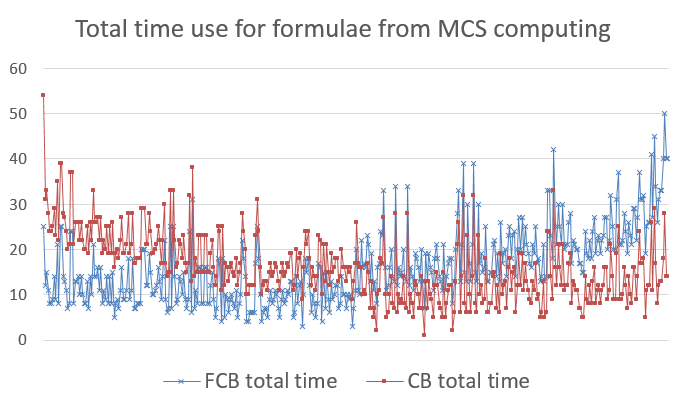
\includegraphics[scale=0.3]{mcs-time.png}
   \caption{Total time use for formulae from MCS computing}
   \label{fig:mcs-time}
\end{figure}

\subsection{Industrial Experimental Results}

For the industrial part, most of the instances were drawn from hardware and software verification. The selection is motivated by the goals of finding instances that contains relatively less clauses and variables and takes a bit longer for SAT solvers to give an implicant. We try to focus on the hard SAT instances because for instances that are easy for SAT solvers, the trivial Test by Variables will be efficiency enough.

In Figure \ref{fig:ind-time}, the total SAT solver time of 104 formulae from industrial track of SAT competition are plotted. The backbones in industrial and practical instances are usually sparse. The experiments results indicate that for most formulae, MEB doesn't need more time than CB does. For some of the formulae, CB need more time than MEB does. It means that in the aspect of time cost, MEB and CB are compatible. The following experiments will show that MEB needs less SAT calls number than CB does on average.

This is because that both CB and MEB requires iterations of SAT solver calls. The SAT solvers computation spent most of CPU time in backbones extraction. If the CPU time of each SAT solver calls is relatively short, there are less possibilities that the instance will become easier. In general, there are more than one model for a satisfiable formula, CB will performs really fast if the model it got from MINISAT randomly suit the algorithm quite well, i.e., for most of the iterations, MINISAT always returns a core that only have one literal. In such cases, CB is faster than MEB.

\begin{figure}
    \centering
    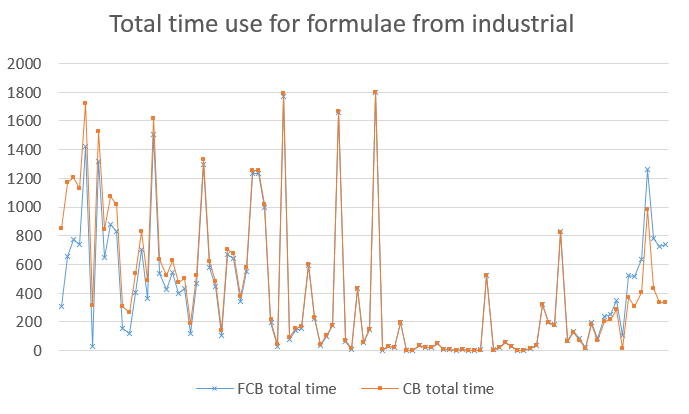
\includegraphics[scale=0.3]{ind-time.png}
   \caption{Total time use for formulae from industrial}
   \label{fig:ind-time}
\end{figure}

\subsection{Fixed Percentage Experiments Results}

For the fixed percentage part, we take advantages from the CBS family with a fixed backbones percentage of 10\%, 30\%, 70\% and 90\% respectively, also from SATLIB.
For each group of the fixed backbone percentage instances, there are 1000 instances in the group.

With the simply instances, it's sufficient to evaluate the efficiency of algorithms by only calculate the SAT calls number.
Figure \ref{fig:fix} illustrates the SAT call numbers needed by MEB and CB for different percentages. It's obvious that for most of the instances, MEB need less SAT call numbers than CB does, despite the percentage of backbones. It proves that MEB is compatible to CB no matter the backbones are dense or not from the SAT calls number perspective.
\begin{figure} \centering
  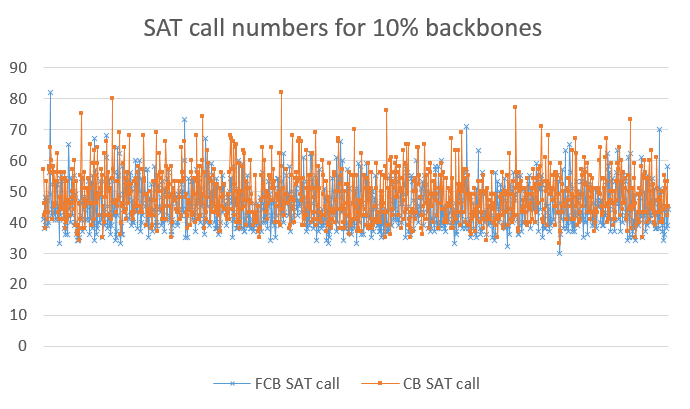
\includegraphics[width=.5\linewidth-0.45mm]{bb-10.png}\hfill
  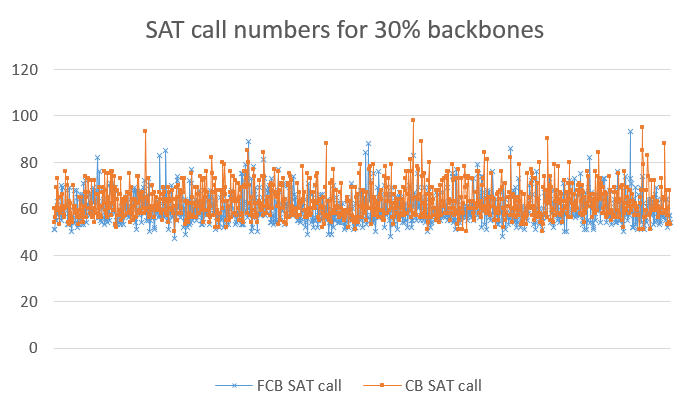
\includegraphics[width=.5\linewidth-0.45mm]{bb-30.png}\\[0.5mm]
  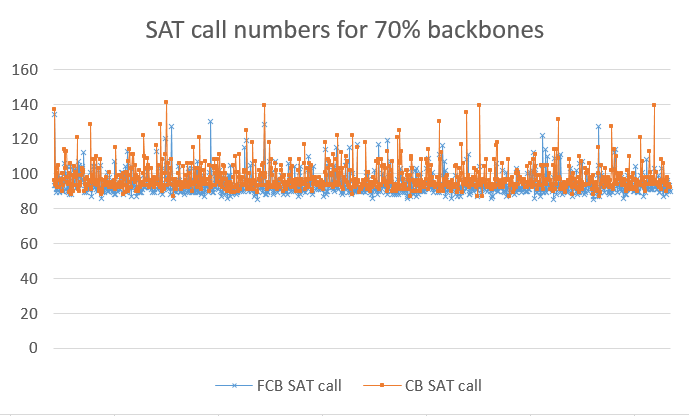
\includegraphics[width=.5\linewidth-0.25mm]{bb-70.png}\hfill
  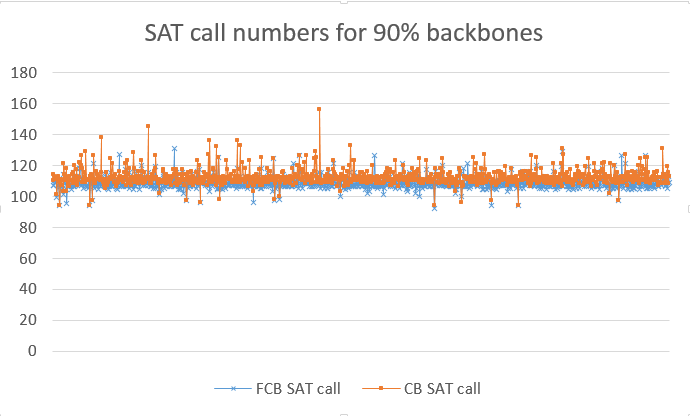
\includegraphics[width=.5\linewidth-0.25mm]{bb-90.png}

    \caption{Total SAT calls number for fixed percentages of backbones formulae}
   \label{fig:fix}
\end{figure}

The results reveal that MEB is as efficiency as CB in general. For dense backbones formulae, MEB needs less total SAT solver time. The experiment results present that MEB outperforms CB with MSS formulae that generated from unsatisfiable formulae. It's because that MEB is more efficient when dealing with dense backbones. As a result, for dense backbones, MEB is better, no matter the formula is from MSS computing, practical verification or crafted.
As discussed above, for unsatisfiable formulae, the density of backbones will increase simultaneously with the size of MSS formula. In the application of hardware model checking, planning and fault localization, the backbones are dense. With a proper use of other techniques, MEB will reach better performance in application.




